\chapter{Testy}
\label{rozdzial4}

\par Podczas procesu tworzenia kompilatora, były również tworzone programy testujące dla poszczególnych funkcjonalności, w celu zweryfikowania prawidłowego działania programu. Dla każdego z modułów został utworzony program testujący w języku JavaScript, który obejmuje zakres funkcjonalności modułu. Zostały również utworzone tożsame programy w języku C\# w celu porównania do kodu języka JavaScript.
\par Zostały również wykorzystane dwa gotowe programy napisane w JavaScript odnalezione w Internecie. Również dla tych programów zostały utworzone odpowiedniki w języku C\# oraz zostały stworzone programy w języku JScript. Dla programów zostały przeprowadzone dodatkowe testy: został zmierzony czas wykonywania programu, zużycie pamięci oraz wielkości pliku wynikowego.

\section{Testy modułów}

\par A

\subsection{Porównanie wyniku wykonania programów}

\par Pierwszym z testów został wykonany program testujący wyświetlanie elementów na ekranie. Program wyświetla różne wartości różnych typów, takie jak wartości tekstowe w cudzysłowu podwójnym jak i pojedynczym, wartości liczbowe całkowite i rzeczywiste, wartości logiczne oraz tablice wartości. Na załączonym rysunku \ref{fig:result1} przedstawione są zrzuty ekranu wyniku działania programów w różnych wariantach.

\begin{figure}[!h]
	\centering
  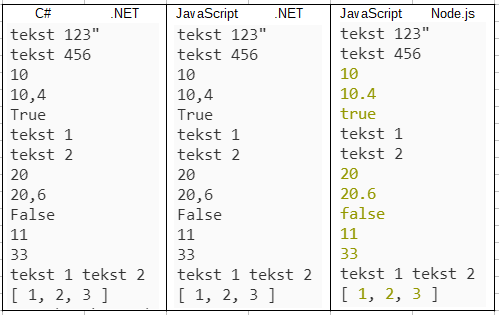
\includegraphics[width=0.7\linewidth]{t1.png}
	\caption{Wyniki wykonania programu testowego dla modułu obsługi standardowego wyjścia. Źródło: własne}
	\label{fig:result1}
\end{figure}

\par Jak można zauważyć, wynik programu w języku C\# oraz JavaScript kompilowanych na wspólną platformę .NET są identyczne. Tutaj należy również wspomnieć, że standardowa biblioteka C\# nie posiada, żadnej z funkcji pozwalającej na wyświetlenie listy elementów tablicy przy pomocy jednej instrukcji. Tak jak podczas implementacji kompilatora JavaScript została zastosowana tutaj funkcja łącząca elementy tablicy w jeden ciąg znaków oraz zostały doklejone nawiasy otwierające oraz zamykające. 
\par Porównując wynik programu uruchomionego na platformie .NET z programem uruchomionym na platformie Node.js, można zauważyć nie wielkie różnice w wyświetlanych wynikach. Pierwszą z nich rzucającą się w oczy, jest zmiana koloru wyświetlanego tekstu dla liczb oraz wartości liczbowych. Jednak ten efekt zależny jest od formatowania kolorów w danej konsoli. Konsola wykryła wywołanie platformy Node.js, dzięki czemu zmieniła kolorystykę.
\par Drugim z różniącym się elementem jest sposób wyświetlania liczb rzeczywistych. Różnią się tym, że dla platformy .NET wyświetlany jest przecinek, kiedy na platformie Node.js wyświetlana jest kropka. Ostatnią różnicą w prezentowanych wynikach jest wyświetlanie wartości logicznych. Dla platformy .NET wartości są wyświetlane z wielką literą, a w przypadku Node.js wartości wyświetlane są małymi literami.

\par Kolejnym z testów dla którego wynik wykonania programu był różny, został przeprowadzony dla modułu działań arytmetycznych. Zrzuty wyników zostały przedstawione na rysunku \ref{fig:result2}. Głównie różnice występują przy wyświetlaniu wyniku operacji dzielenia.

\begin{figure}[!h]
	\centering
  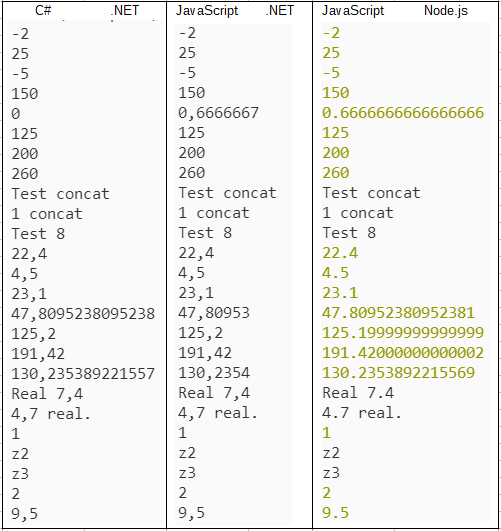
\includegraphics[width=0.7\linewidth]{t2.png}
	\caption{Wyniki wykonania programu testowego dla modułu obsługi działania arytmetyczne. Źródło: własne}
	\label{fig:result2}
\end{figure}

\par Pierwszą z różnic między programem napisanym w języku C\# a JavaScript na platformie .NET jest wynik dzielenia dwóch liczb całkowitych. Wykonywane działanie ma postać $y = 10 / 15$, więc wynikiem jest liczba rzeczywista. W programie w języku C\# jest językiem silnie typowanym, co oznacza, że jeżeli przynajmniej jedna z liczb nie zostanie przekonwertowana na typ liczb rzeczywistych, to wynik będzie typu liczby całkowitej. W tworzonym kompilatorze została zaimplementowana automatyczna konwersja typów, w momencie kiedy zostanie wykryta operacja dzielenia dwóch liczb.
\par Drugą z widocznych różnic jest precyzja wartości zmiennych. W tworzonym kompilatorze JavaScript został wykorzystany typ pojedynczej precyzji, a w przypadku kompilatora C\# została zastosowana typ podwójnej precyzji. Porównując wyniki platformy .NET do platformy Node.js można zauważyć, że wartości na platformie .NET są zaokrąglane.

\par Przy uruchomieniu programu JScript jednego z algorytmów testujących, ukazała się jeszcze jedna różnica w prezentowanych na konsoli wynikach. Różnicą jest sposób wyświetlania tablicy elementów. W tworzonym kompilatorze, jak i na platformie .NET, elementy są otoczone nawiasem kwadratowym, oraz oddzielone są poza przecinkiem dodatkową spacją. W przypadku wyniku programu JScript, prezentowana tablica nie posiada nawiasów kwadratowych oraz liczby są oddzielone przecinkami bez spacji. Wynik programów zaprezentowany jest na rysunki \ref{fig:result3}

\begin{figure}[!h]
	\centering
  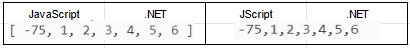
\includegraphics[width=0.7\linewidth]{t3.png}
	\caption{Wyniki wykonania programu dla algorytmu testowego nr 1. Źródło: własne}
	\label{fig:result3}
\end{figure}

\par Skrypty testowe dla pozostałych modułów nie wykazują różnic w prezentowanych wynikach na konsoli.

\subsection{Porównanie generowanego kodu assemblera}

\par Generowany kod assemblera z języka JavaScript będzie porównany z kodem dezasemblowanym kodem programu napisanego w języku C\#. Dezasemblacja jest wykonywana przy pomocy programu \textit{ildasm.exe} znajdujący się w pakiecie \textbf{.NET Framework}.
\par Pierwszą z widocznych różnic jest ilość deklaracji metadanych w nagłówku pliku. Kolejną z różnic jest ilość modyfikatorów przy deklaracji klasy jak i metody \texttt{Main}. Dla deklaracji klasy programu C\# zostały użyte następujące słowa kluczowe \texttt{private}, \texttt{auto}, \texttt{ansi}, \texttt{beforefieldinit}, a dla funkcji \texttt{Main} zostały użyte: \texttt{private} oraz \texttt{hidebysig}. 

\begin{figure}[!h]
	\centering
  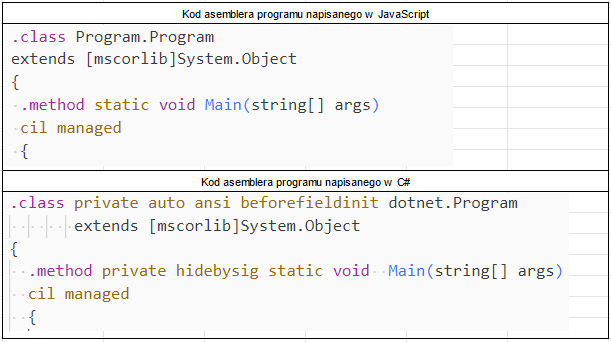
\includegraphics[width=0.9\linewidth]{t4.png}
	\caption{Porównanie kodu asemblera dla deklaracji klasy oraz funkcji \texttt{Main}. Źródło: własne}
	\label{fig:result4}
\end{figure}

\par Kolejnym z różnic jest ilość deklarowanych zmiennych, która spowodowana jest słabą optymalizacją w tworzonym kompilatorze. Następną rzeczą jest nadawanie etykiet dla każdej z instrukcji w obrębie deklarowanych funkcji. 

\par Analizując generowane instrukcje kodu asemblera z dezasemblowanym kodem programu C\# można zauważyć różnicę przy zapisywaniu oraz odczytywaniu wartości zmiennych na stosie. W utworzonym kompilatorze odbywa się to zawsze poprzez nazwę zmiennej, a w .NET Framework wykorzystywane są instrukcje wykorzystujące indeksowanie zmiennych od wartości 0 do 3. Dodatkowo odwołanie się do kolejnych zmiennych wykorzystywana jest instrukcja w formie skróconej.


\begin{lstlisting}[language=IL, caption={Fragment kodu deasemblerowanego testu programu C\#, przedstawiający ładowanie wartości zmiennych na stos}, label=alg:asm]
  ...
  IL_0047:  ldloc.0
  IL_0048:  call       void [mscorlib]System.Console::WriteLine(string)
  IL_004d:  ldloc.1
  IL_004e:  call       void [mscorlib]System.Console::WriteLine(string)
  IL_0053:  ldloc.2
  IL_0054:  call       void [mscorlib]System.Console::WriteLine(int32)
  IL_0059:  ldloc.3
  IL_005a:  call       void [mscorlib]System.Console::WriteLine(float32)
  IL_005f:  ldloc.s    V_4
  IL_0061:  call       void [mscorlib]System.Console::WriteLine(bool)
  ...
\end{lstlisting}

\par Następne różnice generowanego kodu widoczne są przy operacjach arytmetycznych, wykonywanych na liczbach stałych. W przypadku wykorzystania \textit{.NET Framework}, obliczenia wykonywane są przy generowaniu kodu, a nie podczas uruchomienia skompilowanego programu. Przykładowo wykonanie działania $x = 1 + 2$, wygeneruje instrukcje jedynie do przypisania wartości $3$ do zmiennej $x$. W tworzonym kompilatorze, wygenerowanie zostanie instrukcji do załadowania liczby $1$ oraz $2$ na stos, następnie wykonanie operacji dodawania i na końcu przypisanie wyniku do zmiennej $x$.
\par Przy dodawaniu do siebie wielu łańcuchów znaków, w kodzie assemblera, programu napisanego w języku C\#, można zauważyć, że wszystkie łańcuchy są łączone przy pomocy jednej instrukcji \texttt{Concat}, gdzie w tworzonym kompilatorze, zawsze łączone są jedynie dwa łańcuchy na raz. Co więcej, można zauważyć też różnicę przy konwersji wartości zmiennych na łańcuchy znaków przy dodawaniu ich do elementów typu łańcuchowego. W tworzonym kompilatorze konwersja przebiega przy pomocy instrukcji \texttt{ToString()}, jednak w kompilatorze środowiska \textit{.NET Framework} przeprowadzana jest przy pomocy instrukcji \texttt{box}, która sprowadza zmienną do typu \texttt{object}. Instrukcja \texttt{Concat} przyjmuje wtedy elementy typu \texttt{object}.

\begin{lstlisting}[language=IL, caption={Fragment kodu deasemblerowanego testu programu C\#, przedstawiający łączenie łańcuchów znaków}, label=alg:asm]
  ...
  IL_006a:  ldloc.s    V_1
  IL_006c:  ldc.i4.2
  IL_006d:  box        [mscorlib]System.Int32
  IL_0072:  ldstr      "Tekst"
  IL_0077:  call       string [mscorlib]System.String::Concat(object,
                                                              object,
                                                              object)
  ...
\end{lstlisting}

%  instrukcje warunkowe wykorzystują różne rodzaje skoków, gdzie u mnie jest zawsze sprowadzane do boolean

% Do sprawdzenia: pętle, tablice, funkcje


% 1. Obsługa standardowego wyjścia
% 2. Obsługa zmiennych
% 3. Obsługa działań arytmetycznych
% 4. Obsługa wyrażeń warunkowych
% 5. Obsługa pętli
% 6. Obsługa tablic
% 7. Obsługa funkcji

% \section{Testy algorytmów}

% \section{Proste operacje matematyczne}
% Test dodawania, odejmowania, mnożenia, dzielenia, przypisywania.
% \section{Kolejność wykonywania działań}
% Test na bardziej złożonych wyrażeniach. Sprawdzenie poprawności działania nawiasów oraz kolejności wykonywania działań.
% \section{Wyrażenia warunkowe}
% Test wyrażeń warunkowych. Kolejność wykonywania operacji and i or.
% \section{Tablice}
% Test obsługi tablic jedno i wielowymiarowych.
% \section{Obiekty}
% Test obsługi obiektów.
% \section{Klasy}
% Jeśli będzie implementacja.
% Test działania obiektów klas.
% \section{Funkcje}
% Test działania funkcji.
% 1. Funkcja "void" bez parametrów.
% 2. Funkcja "void" z parametrami.
% 3. Funkcja zwracająca różne typy (proste, tablice, obiekty) bez parametrów.
% 4. Funkcje zwracająca różne typy z parametrami.
% 5. inne

% \section{Algorytm 1}
% \subsection{Opracowanie pseudokodu algorytmu 1}
% \subsection{Implementacja algorytmu 1}
% \subsection{Testy algorytmu 1}
% \section{Algorytm 2}
% \subsection{Opracowanie pseudokodu algorytmu 2}
% \subsection{Implementacja algorytmu 2}
% \subsection{Testy algorytmu 2}
